% !TEX TS-program = pdflatex
% !TEX encoding = UTF-8 Unicode

% This is a simple template for a LaTeX document using the "article" class.
% See "book", "report", "letter" for other types of document.

\documentclass[12pt]{article} % use larger type; default would be 10pt

\usepackage[utf8]{inputenc} % set input encoding (not needed with XeLaTeX)

%%%%\usepackage[document]{ragged2e} 

%%% Examples of Article customizations
% These packages are optional, depending on whether you want the features they provide.
% See the LaTeX Companion or other references for full information.

%%% PAGE DIMENSIONS
\usepackage{geometry} % to change the page dimensions
\geometry{letterpaper} % or letterpaper (US) or a5paper or....
\geometry{margin=1in} % for example, change the margins to 2 inches all round
% \geometry{landscape} % set up the page for landscape
%   read geometry.pdf for detailed page layout information

\usepackage{graphicx} % support the \includegraphics command and options
\graphicspath{
{figs/ipe/}
}
% \usepackage[parfill]{parskip} % Activate to begin paragraphs with an empty line rather than an indent

%%% PACKAGES
\usepackage{booktabs} % for much better looking tables
\usepackage{array} % for better arrays (eg matrices) in maths
\usepackage{paralist} % very flexible & customisable lists (eg. enumerate/itemize, etc.)
\usepackage{epstopdf}
\epstopdfsetup{suffix = {}}
\usepackage{siunitx}
\sisetup{unitsep = \cdot}
\usepackage{verbatim} % adds environment for commenting out blocks of text & for better verbatim
\usepackage{subfig} % make it possible to include more than one captioned figure/table in a single float
% These packages are all incorporated in the memoir class to one degree or another...

\usepackage{caption}        %Allows modification of captions
% \usepackage{indentfirst}    %Allows for indenting first paragraphs



\usepackage{hyperref}
\usepackage{todonotes}

%%% HEADERS & FOOTERS
\usepackage{fancyhdr} % This should be set AFTER setting up the page geometry
\pagestyle{fancy} % options: empty , plain , fancy
\renewcommand{\headrulewidth}{0pt} % customize the layout...
\lhead{}\chead{}\rhead{}
\lfoot{}\cfoot{\thepage}\rfoot{}

%%% SECTION TITLE APPEARANCE
\usepackage{sectsty}
\usepackage{tikz}
\usepackage[framemethod=TikZ]{mdframed}
\usepackage{enumerate}
\allsectionsfont{\sffamily\mdseries\upshape} % (See the fntguide.pdf for font help)
% (This matches ConTeXt defaults)

%%% ToC (table of contents) APPEARANCE
\usepackage[nottoc,notlof,notlot]{tocbibind} % Put the bibliography in the ToC
\usepackage[titles,subfigure]{tocloft} % Alter the style of the Table of Contents
\renewcommand{\cftsecfont}{\rmfamily\mdseries\upshape}
\renewcommand{\cftsecpagefont}{\rmfamily\mdseries\upshape} % No bold!

%%% END Article customizations

%%% The "real" document content comes below...

\title{Robotic Cart System}
\author{Kalli Allen, Darrah Beebe, and Jason Braker \\ \underline{Advisor}: Dr. Suruz Miah}

%\date{} % Activate to display a given date or no date (if empty),
         % otherwise the current date is printed 
         
% \setlength{\parindent}{4em} % this should indent paragraphs

\begin{document}
\maketitle

\section{Project Description}
Robotic carts are of paramount importance to conduct many indoor or outdoor tasks. There are many applications of autonomous robotic carts. For example, in a grocery store, a customer (especially a person with disability) may need more than one cart but is incapable of pushing two carts simultaneously. Therefore, a second cart that is capable of identifying the customer to follow and is able to track and follow the customer through the store would be very useful. In an indoor office environment, such an autonomous robotic cart may be used to carry items such as files from one office to another. In an outdoor environment, such a cart may be used to carry sheets of glass.

There are many solutions available in the market for such robotic carts. However, all of them require line of sight communication. In this project, we are proposing a robotic cart using mainly analog signals using cost-effective wireless communication. Implementation of a fully functional robotic cart will be out of the scope of this project but is an ultimate goal for this project in the coming years. However, this project is expected to encourage further research in this area as well as provide a foundation for that research.

%------------------------------------------------
\section{System Architecture}
\subsection{System Block Diagram}
The robotic cart system will be comprised of two main subsystems - a mobile cart and a remote target device. \textlangle Darrah's block description here\textrangle

A block diagram of the robotic cart system is shown in \autoref{fig:sysBlockDiag}
\begin{figure}
    \centering
    \captionsetup{justification=centering, margin=3cm}
    % Uncomment the below line once Kalli's block diagram figure is included in the figs folder
    % 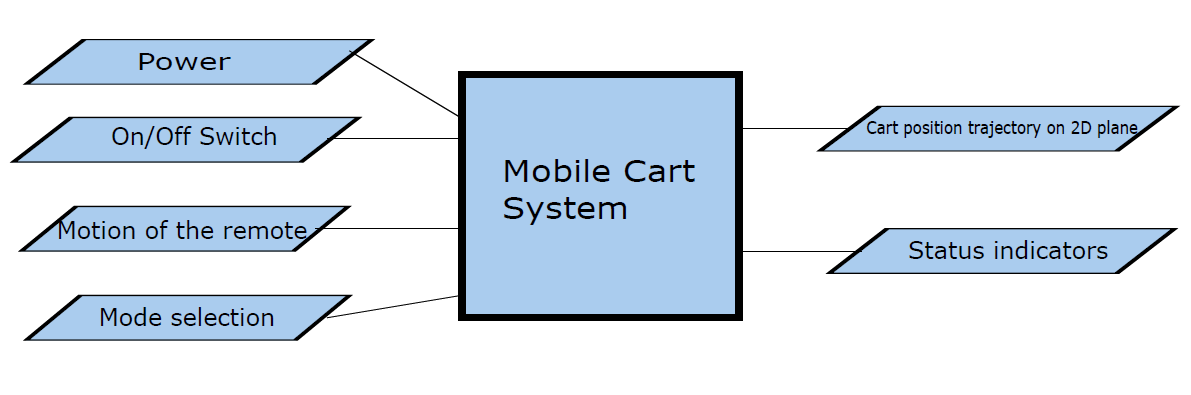
\includegraphics{figs/img/sysBlockDiag}
    \caption{Block Diagram of the Robotic Cart System}
    \label{fig:sysBlockDiag}
\end{figure}

\subsection{System Inputs and Outputs}
\subsubsection{Inputs}
There are four inputs to the robotic cart system.
\begin{enumerate}
    \item Power - Both the mobile cart and the remote will require power from a battery.
    \item On/Off Switch - The user must be able to turn both the cart and the remote off to save power when the robotic cart system is not in use.
    \item Movement of the Remote - The user will control the mobile cart by moving with the remote.
    \item Mode Selection - The user must be able to select which mode of operation the robotic cart system should use.
\end{enumerate}

\subsubsection{Outputs}
There are two outputs from the robotic cart system.
\begin{enumerate}
    \item Cart Position Trajectory on 2D Plane - The cart will move to follow the remote.
    \item Status Indicators - Both the mobile cart and the remote will have status indicators to provide the user with the status of the system.
\end{enumerate}

%------------------------------------------------
\section{Requirements and Specifications}
\subsection{Requirements}
The robotic cart system will meet the following requirements:
\begin{enumerate}
    \item Cart must follow remote at a reasonable distance
    \item Cart must be able to travel at a speed reasonable for walking
    \item User must be alerted if cart falls too far behind
    \item Cart must not require line-of-sight to follow remote
    \item Cart must avoid obstacles
\end{enumerate}

\subsection{Specifications}
Based on the requirements, the robotic cart system must meet the following specifications:
\begin{enumerate}
    \item Cart must be able to follow the remote while maintaining a distance of 1 to 1.5 meters.
    \item Cart must be able to travel at 2 m/s
    \item User must be alerted if the cart falls more than 2 meters behind
    \item Cart must be not require line-of-sight to follow remote
    \item Cart must not collide with obstacles while following remote
\end{enumerate}

% %Each of the helicopters we will be using have fixed bases as shown in \autoref{fig:QuanserAero} (courtesy of Quanser Inc.).

% Each of the helicopters used will have fixed bases as shown in \autoref{fig:QuanserAero} (courtesy of Quanser Inc.).  

% \begin{figure}
%   \centering
%   \captionsetup{justification=centering,margin=3cm}
%   \includegraphics{figs/img/QuanserAero}
%   \caption{Quanser Aero 2-DOF Helicopter \newline (\url{https://www.quanser.com/products/quanser-aero/})}
%   \label{fig:QuanserAero}
% \end{figure}
% %
% The tail of the helicopter has a motor that controls its yaw motion.  Similarly, the main rotor changes the pitch of the helicopter.  The directions in which the motors spin will be determined by the polarity of the applied voltages.  This will be regulated by our smart control algorithm.


% \section{Modes of Operations}
% %\label{sec:modesOfOperations}
% We plan on allowing the user to control the helicopter using three modes of operation.  A short description of each mode is given below.

% \begin{enumerate}[\textbf{Mode~\#}1:]
%     \item Allows the user to control the helicopters to a given configuration. For example, setting the pitch to 45 degrees and the yaw to 90 degrees will move the helicopter that much from the initial configuration.
%     \item Allows the user to choose a time varying input signal, so the helicopter will have a wave-like motion shifting from one configuration to another.  Examples include sine and square waves.
%     \item Allows the user to control the algorithm that the user wishes to apply.  They will be able to choose from LQR, LQG, or ADP.
% \end{enumerate}

\end{document}

%%% Local Variables:
%%% mode: latex
%%% TeX-master: t
%%% End:
